
%%\documentclass[referee,sn-basic]{sn-jnl}% referee option is meant for double line spacing

%%=======================================================%%
%% to print line numbers in the margin use lineno option %%
%%=======================================================%%

%%\documentclass[lineno,pdflatex,sn-basic]{sn-jnl}% Basic Springer Nature Reference Style/Chemistry Reference Style


%\documentclass[pdflatex,sn-mathphys-num]{sn-jnl}% Math and Physical Sciences Numbered Reference Style
%%\documentclass[pdflatex,sn-mathphys-ay]{sn-jnl}% Math and Physical Sciences Author Year Reference Style
%%\documentclass[pdflatex,sn-aps]{sn-jnl}% American Physical Society (APS) Reference Style
%%\documentclass[pdflatex,sn-vancouver-num]{sn-jnl}% Vancouver Numbered Reference Style
%%\documentclass[pdflatex,sn-vancouver-ay]{sn-jnl}% Vancouver Author Year Reference Style
\documentclass[pdflatex,sn-apa]{sn-jnl}% APA Reference Style
%%\documentclass[pdflatex,sn-chicago]{sn-jnl}% Chicago-based Humanities Reference Style

%%%% Standard Packages
%%<additional latex packages if required can be included here>

\usepackage{graphicx}%
\usepackage{multirow}%
\usepackage{amsmath,amssymb,amsfonts}%
\usepackage{amsthm}%
\usepackage{mathrsfs}%
\usepackage[title]{appendix}%
\usepackage{xcolor}%
\usepackage{textcomp}%
\usepackage{manyfoot}%
\usepackage{booktabs}%
\usepackage{algorithm}%
\usepackage{algorithmicx}%
\usepackage{algpseudocode}%
\usepackage{listings}%
\usepackage{tikz}
\usetikzlibrary{shapes.geometric, arrows.meta, positioning, calc}
%%%%

\raggedbottom
%%\unnumbered% uncomment this for unnumbered level heads

\begin{document}

\title[AI Disaster Opinions and Action]{Breaking the Bubble? AI’s Role in Shaping Disaster Opinions and Driving Social Action}

%%=============================================================%%
%% GivenName	-> \fnm{Joergen W.}
%% Particle	-> \spfx{van der} -> surname prefix
%% FamilyName	-> \sur{Ploeg}
%% Suffix	-> \sfx{IV}
%% \author*[1,2]{\fnm{Joergen W.} \spfx{van der} \sur{Ploeg} 
%%  \sfx{IV}}\email{iauthor@gmail.com}
%%=============================================================%%

\author*[1, 2]{\fnm{Tina} \sur{Comes}}\email{t.comes@tudelft.nl}

\affil*[1]{\orgdiv{Faculty Technology, Policy \& Management}, \orgname{TU Delft}, \orgaddress{ \city{Delft}, \country{The Netherlands}}}

\affil[2]{\orgdiv{Institut for the Protection of Terrestrial Infrastructures}, \orgname{DLR}, \orgaddress{ \city{Sankt Augustin}, \country{Germany}}}

%%==================================%%
%% Sample for unstructured abstract %%
%%==================================%%

\abstract{Crises change human information collection, sharing, and decision-making. The combination of urgency, uncertainty, and high-stakes is known to induce cognitive biases, informational bubbles and echo chambers. Trustworthy Artificial Intelligence (AI) promises solutions to optimise decisions and reduce informational bottlenecks. Yet, introducing AI as a 'trusted' actor in crises fundamentally changes human interaction, information processing and decision-making. While the literature on Human-Centred AI often focuses on the impact of an AI on individual biases or decisions, what is missing is an understanding at scale how AI shapes information processing, opinions and decisions during volatile and uncertain conditions as typical for disasters.

This paper uses an agent-based model (ABM) to explore how AI impacts information processing, sharing and decision-making during crises, especially if that AI seeks to gain trust by tuning into human beliefs. To explore the effects for different prototypical behaviours, the human agents in the ABM adopt exploratory or exploitative behaviours modelled through Q-learning algorithms and update their beliefs using Bayesian techniques. 

Our findings reveal nuanced interactions: AI can initially improve situational awareness, it often inadvertently introduces or reinforces new echo chambers and interrupts social networks. Identifying tipping points where AI transitions from mitigating to amplifying filter bubbles provides critical insights to understand how to balance use of AI and accuracy, and how much inaccuracy might be needed.}

\keywords{Disaster Response, AI for Good, Opinion Dynamics, Filter Bubble, Echo Chamber, Opinion-Action Dynamic, Hybrid Intelligence}

%%\pacs[JEL Classification]{D8, H51}

%%\pacs[MSC Classification]{35A01, 65L10, 65L12, 65L20, 65L70}

\maketitle

\section{Introduction}\label{sec1}
Increasingly, we humans rely on artificial intelligence (AI) to collect and analyse information and make decisions \citep{klingbeil2024trust}. This trend is particularly pronounced during crises, where decision-makers are confronted with highly complex decisions that need to be addressed urgently, leaving limited time for reflection and deliberation \citep{mendonca2001decision}. This combination is known to deeply impact human information processing, sharing decision-making behaviour \citep{comes2020coordination}. To help humans manage this complexity, Artificial Intelligence (AI) is promoted as a tool to optimise decisions and information flows \citep{jeon2024hearhere}. The idea that AI will facilitate immediate access to "objective', 'data-driven' or neutral information, or facilitate interaction with diverse viewpoints is expected to improve situational awareness and prevent fragmentation. 

A prerequisite to the use of technology in crises is trust \citep{steinbrink2024impact}. In the field of AI, there is a plethora of guidelines and approaches that speak to designing AI that is \textit{trustworthy}, especially in the context of crises and disasters -- for a recent review, see \citep{albahri2024systematic}. Often, the trust relationship is conceptualised as one individual trusting one AI, whereby it is claimed that trust is promoted by more transparency \citep{visave2025transparency}. Others focus on \textit{public} trust as a result of a design and decision-making process \citep{tzachor2020artificial}. Recognising that humans -- especially in crises -- have a tendency of selective exposure \citep{barbera2015tweeting}, and confirmation bias \citep{paulus2024interplay}, whereby they reject conflicting information. 

Increasingly, especially generative AI (genAI) has started to mimic human behaviour and tune to the opinions of the human \citep{sharma2024generative}, as a way to gain acceptance and 'trust'. This introduces a fundamental dilemma: should AI provide accurate information—even if it contradicts beliefs and is potentially rejected—or should it align with human beliefs to foster immediate acceptance and trust? If AI overly tunes into existing beliefs to gain rapid trust, it risks amplifying cognitive biases and echo chambers \citep{ekstrom2022self}. Echo chambers are segregated information spaces, in which pre-existing beliefs are reinforced, and there is limited exposure to diverse or contradictory perspectives potentially leading to polarisation \citep{jeon2024hearhere}. The architecture of online informationscapes, together with the increasing personalisation of AI to its user has the potential to contribute to the formation and maintenance of these echo chambers. Conversely, providing correct but contradictory information might lead to information rejection and distrust in AI, whereby social echo chambers and human biases cannot be overcome.

While studies and insights on the implications of black box genAI models have started to emerge \citep{zhang2024see, sharma2024generative}, a gap in current research is understanding how these interactions of individuals with AI scale up to broader social network dynamics during crises, potentially creating or exacerbating polarisation and filter bubbles. This paper addresses a fundamental question: Does AI act as a bridge that breaks echo chambers by providing broader perspectives during crises, or does it instead reinforce existing filter bubbles through its alignment mechanisms?

To start exploring these dynamics, we use an agent-based modelling (ABM) approach that allows us to simulate interactions between heterogeneous human agents and AI during crises. The model simulates decentralised disaster relief efforts where human agents, characterised by distinct behavioural types, interact with human or AI information sources to allocate resources across a spatial environment. This computational approach enables us to observe emergent patterns of information flow, belief formation, and decision outcomes across different network configurations and behavioural strategies. We analyse the trade-off between the adoption and use of AI, and the resulting situational awareness, filter bubbles and decision performance. 

The model expands on established opinion dynamics frameworks \citep{geschke2019triple} to incorporate the challenges of human-AI interaction. To understand the impact of different human behavioural patterns, we analyse two different prototypical human decision-making strategies under uncertainty as a way to manage the trade-off between broad information collection to reduce uncertainty (exploration) and reward seeking within limited local environments (exploitation) - the latter pattern being typical for the responsive short-term focus of crisis management \citep{comes2020coordination}. Information adoption by agents is modelled through Bayesian updating, enabling dynamic belief revision based on new evidence and AI recommendations.

This approach allows us to analyse how different information sources, behavioural patterns and dynamic trust relationships influence collective decision-making in crisis response. The analysis identifies tipping points where the benefits of AI of being able to exploring broader areas transition into detrimental influence by creating new echo chambers. These insights contribute to the ongoing discussions about what constitutes \textit{trustworthy} AI, and how we strike a balance between optimising the adoption and use of the technology versus its impact, particularly in complex, highly dynamic and morally charged situations such as crises.

\section{Background}

Fuelled by climate change, increasing inequalities, conflict and war, we are confronted with global poly-crises that erode progress towards sustainability \citep{sogaard2024evolution}. As crises require rapid interventions that overwhelm human decision-making capacity, digital tools have been portrayed as a potential avenue to automatically collect and analyse data to support or make decisions \citep{qadir2016crisis}. Examples range from community mapping \citep{champlin2023measuring, soden2014crowdsourced}, the use of aerial images, remote sensing, UAVs and digital platforms for better crisis management \citep{voigt2007satellite} to increasing automation of the delivery of aid, facilitated by mobile phone and blockchain technology \citep{coughlan2015forecast, baharmand2019leveraging}. Despite these technological advances, the emergent nature of crises poses challenges for information collection, sharing, and decision-making \citep{turoff2004design, nespeca2020towards}.

To better understand the use of AI in the context of crises, we refer to the information management cycle that distinguishes three mechanisms (i) information collection and verification, (ii) information sharing and dissemination and (iii) information use and decision-making \citep{van2015On}. Table \ref{tab:AIcrisis-overview} provides an overview of the promises and perils of AI for the different information management mechanisms, crucial human behavioural patterns and examples of the use of AI in this context. The following sections examine how AI changes these three mechanisms and underlying social and behavioural structures.

\begin{table}
    \small
    \centering
    \begin{tabular}{p{0.15\textwidth} | p{0.15\textwidth} p{0.17\textwidth}p{0.17\textwidth} p{0.17\textwidth}}
        \hline
        \textbf{Mechanism} & \textbf{Promise of AI} &\textbf{ Peril of AI} & \textbf{Human Behaviour} & \textbf{Example Application}\\ \hline
        Information collection & Real-time large-scale information collection \citep{narmatha2025disaster} & Exclusion of marginalised or digitally invisible groups \citep{coleman2024weaving} & Sensemaking \citep{klein2010rapid} & Crowd sensing \citep{mai2025evaluating}, wild fire monitoring \citep{roy2024multi}\\ \hline
        Information sharing & Facilitate access to diverse sources \citep{jeon2024hearhere} & Sharing confined to closed social networks & Trust and alignment, over-reliance \citep{manzini2024should} & Chatbots \citep{urbanelli2024ermes}\\ \hline
        Decision support &  AI delivering tailored and verified information \citep{zhao2025tailoring}, recommendations, automated decisions & Promoting high alignment \citep{manzini2024should}; (moral) de-skilling \citep{vallor2015moral} & (Group) decisions \citep{comes2024ai}, cognitive biases \citep{paulus2022influence} & Agentic AI \citep{acharya2025agentic}, Early Warning \citep{reichstein2025early}\\ \hline
    \end{tabular}
    \caption{Overview of key mechanisms, promise and perils of AI in crisis management}
    \label{tab:AIcrisis-overview}
\end{table}


\subsection{Information collection: knowing more or knowing better?}
AI in combination with data collection via remote sensing or mobile technologies promises a broader perspective, addressing both network density and information intensity that often lack in human social networks \citep{pan2012crisis}. The promise of real-time data collection, especially in highly dynamic situation, is said to allow decision-makers to identify critical tipping points rapidly, before they occur and crises spiral out of control. For almost two decades, focus in this arena has been on social media and real-time surveillance via mobile phones to rapidly understand sentiment, perception, or human movement patterns \citep{middleton2013real, qadir2016crisis, mai2025evaluating}. Following the rapid progress in remote sensing, there are now also increasingly applications in natural hazard monitoring including floods \citep{zhou2024threshold} or wild fires \citep{roy2024multi}.

However, this broad data collection introduces risks of excluding marginalised or digitally invisible populations \citep{coleman2024weaving}. AI-driven information collection typically reflects existing data infrastructures and connectivity patterns, potentially reinforcing structural biases in crisis response rather than overcoming them.

These technological limitations interact with human sensemaking processes during crises \citep{klein2010rapid}. Sensemaking is a process, by which we humans "\textit{make meaning}", especially in conditions of uncertainty and ambiguity \citep{weick2005organizing}. Importantly, sensemaking is a \textit{social} and identity-forming process, in which shared meanings emerge from interaction \citep{maitlis2010sensemaking}. At the same time, the emergent nature of crises poses challenges for information collection \citep{turoff2004design}, where humans tend to  select information that confirms their initial sensemaking trajectories \citep{barbera2015tweeting} and focus primarily on their immediate vicinity and close groups \citep{comes2020coordination}.

\subsection{Information Sharing: Trustworthy AI?}
The second mechanism in Table \ref{tab:AIcrisis-overview} addresses how information is shared across social and organisational networks during crises. Crises are known to disrupt infrastructures, ranging from telecommunication to mobility networks, leading to fragmented social networks and response \citep{holguin2012unique}. AI promises to facilitate access to diverse information sources, possibly breaking social echo chambers \citep{jeon2024hearhere}, potentially bridging fragmented information spaces and overcoming the echo chambers that naturally form during crises.

In addition, crises disrupt infrastructures and social networks leading to fragmentation \citep{wolbers2018introducing}. Especially the combination of low information volume and density has been shown to lead to silos \citep{pan2012crisis}: the well known echo chambers arise. As a consequence, crisis response often focuses on local or regional impacts -- often driven by the experience of the immediate suffering --, yet neglecting the cascading effects across different geographical areas \citep{sigala2022mitigating}.

Foundational theories in opinion dynamics, such as bounded confidence models \citep{hegselmann2002opinion}, state that individuals are more likely to interact with others whose opinions are within a certain range of their own. In contrast, social influence theories emphasise the role of social networks and the tendency for individuals to align their opinions with those of their peers \citep{friedkin1999social}. This alignment is often reinforced by homophily, i.e., the tendency to associate with others who share similar including beliefs \citep{mcpherson2001birds}.

Human information sharing in crises is guided by strong social networks and inter-human relationships. At the onset of a disaster \textit{swift trust,} based on roles, rules, and risk perception is crucial to efficient decision-making \citep{tatham2010application}. Even though the importance of swift trust is recognised, there is limited evidence on the role of technology in shaping it. \citet{dubey2018big} have shown that 'big data' can support building swift trust among actors in humanitarian supply chain. However, it is not clear how the trust relationships that are vital for human-human interaction in crises are translated to interactions with machines, and how social networks and relationships influence the formation, stability, and performance of teams where humans interact with AI at scale. 

A starting point are the trust-building mechanisms between individuals and AI. Importantly, even though users are aware that they are interacting with a machine, they experience the resulting relationship as a trust relationship \citep{manzini2024should}. The literature on trust and trustworthy AI stresses the need for transparency, reliability and alignment in high-stakes environments \citep{lee2004trust, glikson2020human}.

Transparency has been shown said to foster or undermine public trust towards AI in crisis management \citep{steinbrink2024impact, visave2025transparency}. However, given the potential sensitivity of crises information, it is often unclear how much transparency can be provided and achieved \citep{steinbrink2024impact}. Others have highlighted the role of trust into the creator of an AI \citep{saffarizadeh2024relationship}, yet this is unlikely to be known in the rapidly establishing networks in crisis response. Therefore, reliability and alignment play a key role in crisis management. Reliability is defined as \textit{behaving in accordance with expectations}. Alignment refers to the alignment of values or interests, as represented or expected by the humans and their beliefs. Especially in the field of generative AI and AI assistants, it has been shown that users expect an AI to be aligned with their values and interests, and that this alignment can even lead to strong emotional ties \citep{manzini2024should, kaplan2023trust}. From there, tensions emerge between providing accurate recommendations or recommendations that potentially contradicts prior beliefs for higher trust and acceptance \citep{sharma2024generative, ekstrom2022self}.

\subsection{Decision-Making: Rapid AI recommendations or human consensus?}
A challenge in crises is how to translate uncertain and volatile information into action and coordinated decision-making. AI promises to deliver verified information \citep{zhao2025tailoring}, and rapidly analyse large amounts of data. As such, ideas of using AI to support or even automate decisions is becoming increasingly popular as a way to address the double challenge of complexity and urgency \citep{comes2024ai}. AI-driven decision support tools for anticipatory action and forecast-based financing are said to ensure rapid and reliable interventions \citep{thalheimer2022role}. Sure enough, during crises, humans are particularly prone to simplification strategies and heuristics that may be maladaptive in complex environments \citep{klein2010rapid}. These include confirmation bias, where decision-makers selectively attend to information that confirms pre-existing beliefs; anchoring effects, where initial impressions disproportionately influence subsequent judgments; and framing effects, where the way information is presented impacts decision-making \citep{paulus2022influence}.

The need for group decision-making in crisis contexts introduces additional complexities. While groups benefit from diverse perspectives, crisis conditions often undermine these advantages. The pressure to reach consensus quickly can lead to groupthink and centralisation of authority \citep{driskell1991group}, which lead to a silencing of dissenting voices, especially if they are coming from marginalised or low-status groups. AI systems promise to mitigate these group-level biases by providing external, supposedly objective perspectives that can break entrenched patterns of group polarization \citep{jirovsky2021can}. However, the integration of AI recommendations into group processes creates new dynamics that remain poorly understood.


These dynamics become even more pronounced in the hierarchical structures typical of crisis response organizations. Power differentials within teams influence whose perspectives are privileged and how contradictory information is processed \citep{comes2024ai}. When AI recommendations align with powerful stakeholders, they may be more readily accepted regardless of their accuracy, while valuable insights that challenge established authority may be dismissed. This process can lead to what \citet{vallor2015moral} describes as moral de-skilling, where teams or leaders gradually outsource ethical judgment to technological systems without adequate critical engagement.

A critical tension emerges between optimisation for consensus (and trust) versus optimisation for decision quality. AI systems that primarily aim to facilitate agreement may inadvertently reinforce pre-existing group biases rather than challenging them. Conversely, AI systems that prioritize decision quality by presenting contradictory information risk rejection by the group if they disrupt established social dynamics or challenge dominant narratives \citep{manzini2024should}. In addition, the high alignment to values and preferences creates what \citet{west2025ai} terms the "\textit{alignment paradox}," whereby greater alignment of AI towards values can also lead to potentially greater misuse and distortion: "\textit{more virtuous AI may be more easily made vicious}" \citep{west2025ai}.

An open question is thus how the perspective offered by AI is adopted, if it conflict with the actual or perceived urgent local need. In addition, AI can exacerbate selective exposure and confirmation biases by presenting users with content aligned with their prior interactions and the interests of their social networks. That means, via AI alignment, a self-reinforcing loop is introduced that increasingly insulates individuals within homogeneous informationscapes. The resulting echo chambers can solidify their beliefs, and lead to misallocation and biased decisions. 

Especially the tendency to focus on the immediate consequences and neglecting complex or long-term feedback \citep{comes2020coordination} are characteristic for human crisis decisions. The combination of urgency and complexity are known to change decision behaviour \citep{klein2010rapid}, introducing selective exposure \citep{barbera2015tweeting} or cognitive and motivational biases \citep{paulus2024interplay}. 

\subsection{Synthesis}
In sum, AI has been portrayed as a 'solution' to address the flaws of human information collection, processing, sharing and decision-making in crises. However, the context of crises also brings about specific challenges to technology and trustworthy AI in the context of information collection, sharing, and decision-making that are only partially covered in the current guidelines and standards \citep{ozmen2023six}. Current AI tools for crisis response are largely myopic, focusing on addressing immediate problems for crisis response, without considering longer term impacts on social fabric, fairness, or environment and carbon footprint \citep{harika2024harnessing}. Further, several researchers have pointed to the fact that if we delegate responsibility for the safety and well-being of our societies to technological systems, there is a critical spiral of loss of human oversight and control \citep{comes2024ai}. Especially the many moral dilemmas that crisis decisions pertain to remain hard to capture and translate to an AI. Across these three mechanisms—information collection, sharing, and decision support—several critical research gaps emerge:

\textbf{From individual to collective dynamics: }While the literature primarily addresses human-AI trust at the individual level, we need to understand of how these interactions scale to network-level dynamics, influencing collective processes such as sensemaking, and how they contribute to polarisation and fragmentation. This gap is particularly pronounced in crisis contexts, where rapidly forming and dissolving networks create unique informationscapes.

\textbf{AI alignment paradox:} The relationship between AI alignment strategies and echo chamber formation remains poorly understood, particularly when AI systems attempt to gain human trust by reflecting existing beliefs. While high alignment may lead to greater information adoption or 'virtuous' AI, it may also -- via the alignment paradox \citep{west2025ai} -- lead to extreme opposites, thereby fostering polarisation and echo chambers it promised to break
 
This paper contributes by using an innovative agent-based modelling approach that explicitly explores these gaps. By systematically analysing tipping points at which AI shifts from reducing to amplifying filter bubbles, it offers nuanced insights on optimizing AI integration into crisis management processes.
Current research addressing the trajectory of human trust in robotic AI suggests that the 
initial trust starts at a low level and develops over time \citep{glikson2020human}.

\section{Results}

Conventionally, crisis management assumes that a broad exploration beyond potentially localised information bubbles improves situational awareness and coordination \citep{comes2020coordination}. However, our results reveal that people with an exploratory strategy are systematically more vulnerable to an AI that aligns to their beliefs than exploiters who rely on local, familiar information that is provided via their social networks. Figure \ref{fig:fig1AIalign} (left panel) shows an increasing mean belief error from an average of 0.17 for alignment of 0 to 0.3 for an alignment of 0.95 as opposed to relatively stable exploiters (MAE ranges from 0.21 for 0 alignment to 0.24 for high alignment). This result shows that the introduction of highly aligning AI reverses conventional assumptions from bounded rationality literature, by which broad exploration reduces uncertainty. In this experimental set-up this can be explained by the explorers' broader information search that increases exposure to aligned AI, making them more susceptible to systematically biased information.

\begin{figure}
    \centering
    
\includegraphics[width=1\linewidth]{Figures/AIAlignmentImpact_box.png}
    \caption{Performance metrics for different levels of AI alignment. Left panel: mean belief error of agent beliefs vs. ground truth. Middle panel: Disaster Response gap - average number of cells with high needs that are not identified. Right panel: Assistance quality - share of tokens that is correctly delivered to high needs-cells. Results for 30 runs.}
    \label{fig:fig1AIalign}
\end{figure}

As expected, this results in an increase of the disaster response gap, with an average gap of about 2 unidentified cells for the low alignment scenarios (0 and 0.25), 6 for an alignment level of 0.5 and 10 and 11.3 for the high alignment scenarios. In addition, also the variability of results grows with higher alignments (expanding box plots), indicating potential path-dependencies where initial beliefs in combination with potential 'lucky hits' in the uncertain disaster space determine success. This phenomenon of divergence across scenarios is absent in classical opinion dynamics models (Hegselmann \& Krause, 2002; Deffuant et al., 2000) which assume belief convergence, essentially because of the underlying disaster and uncertainty dynamics

From this, also assistance quality suffers, see right panel . Explorers show a consistently higher assistance quality. With a non-aligned AI, they achieve an average of 0.85 \% share of tokens correctly delivered. This share decreases rapidly with growing alignment to below 20 \% for the 0.75 and 0.95 alignment scenarios. This degradation challenges the AI-for-good narrative, whereby AI improves humanitarian response. The finding empirically demonstrates West \& Aydin's (2025) "alignment paradox" in actionable terms: more aligned (ostensibly more "trustworthy") AI produces worse collective outcomes.

\begin{figure}
    \centering
    
\includegraphics[width=0.75\linewidth]{Figures/Fig2_summary_EchoChambers.png}
    \caption{Impact of AI Alignment on Echo Chamber indices}
    \label{fig:fig2_ECHOChambers}
\end{figure}

As a next step, Figure \ref{fig:fig2_ECHOChambers} investigates the underlying belief dynamics and the formation of Echo chambers related to social contexts (Social Echo Chamber Index, SECI) or AI (AI Echo Chamber Index, AECI). Both measure the belief variance within a network of friends or AI reliant agents versus the global belief variance in the network. 

Figure 2 clearly shows that with higher AI alignment both Social and AI-related echo chambers become stronger. The top left corner shows that for low levels of AI alignment (0 and 0.25) exploiters have a better SECI score than explorers (-0.6/-0.1 for an alignment of 0 and -0.1 vs. -0.14 for an alignment of 0.25), indicating that the truthful AI also corrects human beliefs over time. The medium alignment of 0.5 forms a tipping point, where the echo chambers for both agent types are limited to -0.09. For higher levels of AI aligment, AI reinforces social echo chambers by aligning to existing human beliefs: for both agent types, in that case, the SECI moves to less than -0.18. This evolution is reflected by a similar pattern of the AI-reliant group of agents, where for low levels of alignment AI diversifies beliefs (indicated by a positive mean AECI of 0.018 and 0.003 for alignment of 0 and 0.25 respectively), and then also creates increasingly strong echo chambers, with a final mean AECI of -0.05 for the highest alignment. 

The lower panel in Figure 2 shows that this evolution happens even though the call patterns, and the sources that agents query dramatically change. 

\begin{figure}
    \centering
    
\includegraphics[width=0.75\linewidth]{Figures/Fig2_SocialEchoChambers.png}
    \caption{Evolution of Social Echo Chambers over Time}
    \label{fig:fig3_seci}
\end{figure}

\begin{figure}
    \centering
    
\includegraphics[width=0.75\linewidth]{Figures/Fig3_Aeci.png}
    \caption{AI-driven Echo Chambers}
    \label{fig:fig4aeci}
\end{figure}

\begin{figure}
    \centering
    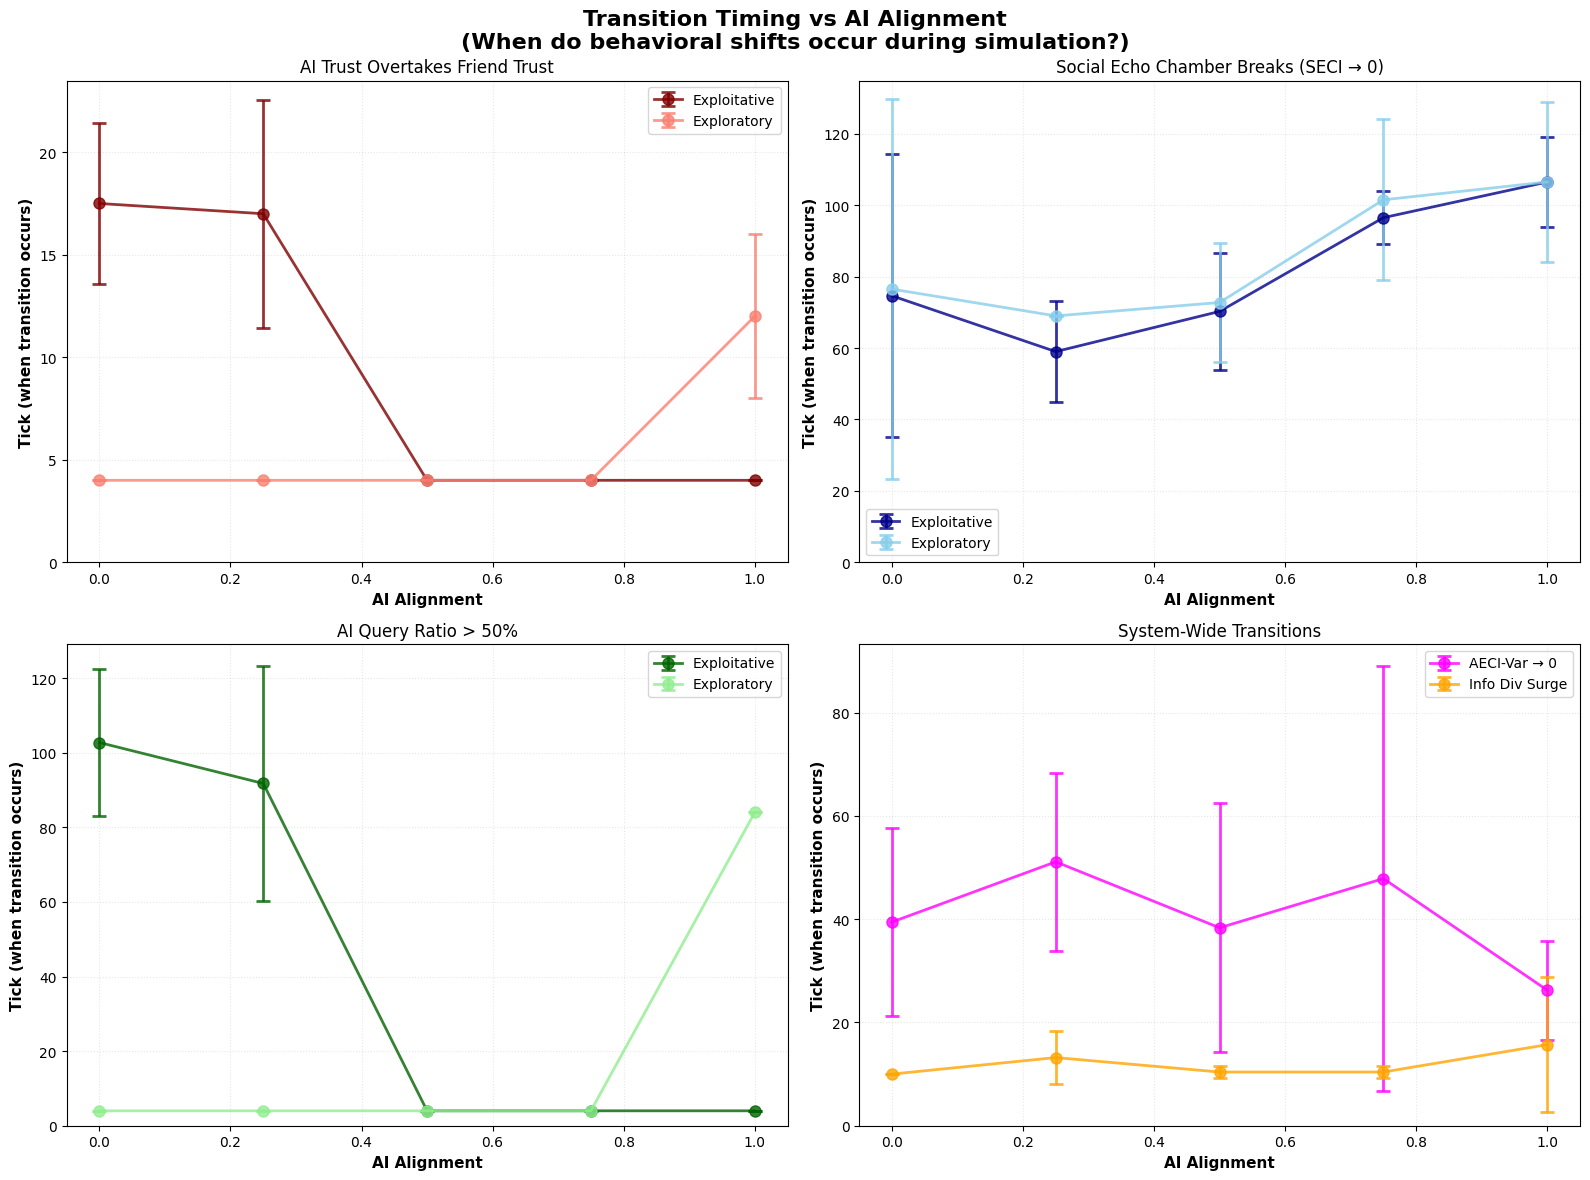
\includegraphics[width=0.5\linewidth]{Fig1_infoDivSurge.png}
    \caption{Enter Caption}
    \label{fig:placeholder}
\end{figure}


\begin{figure}
    \centering
    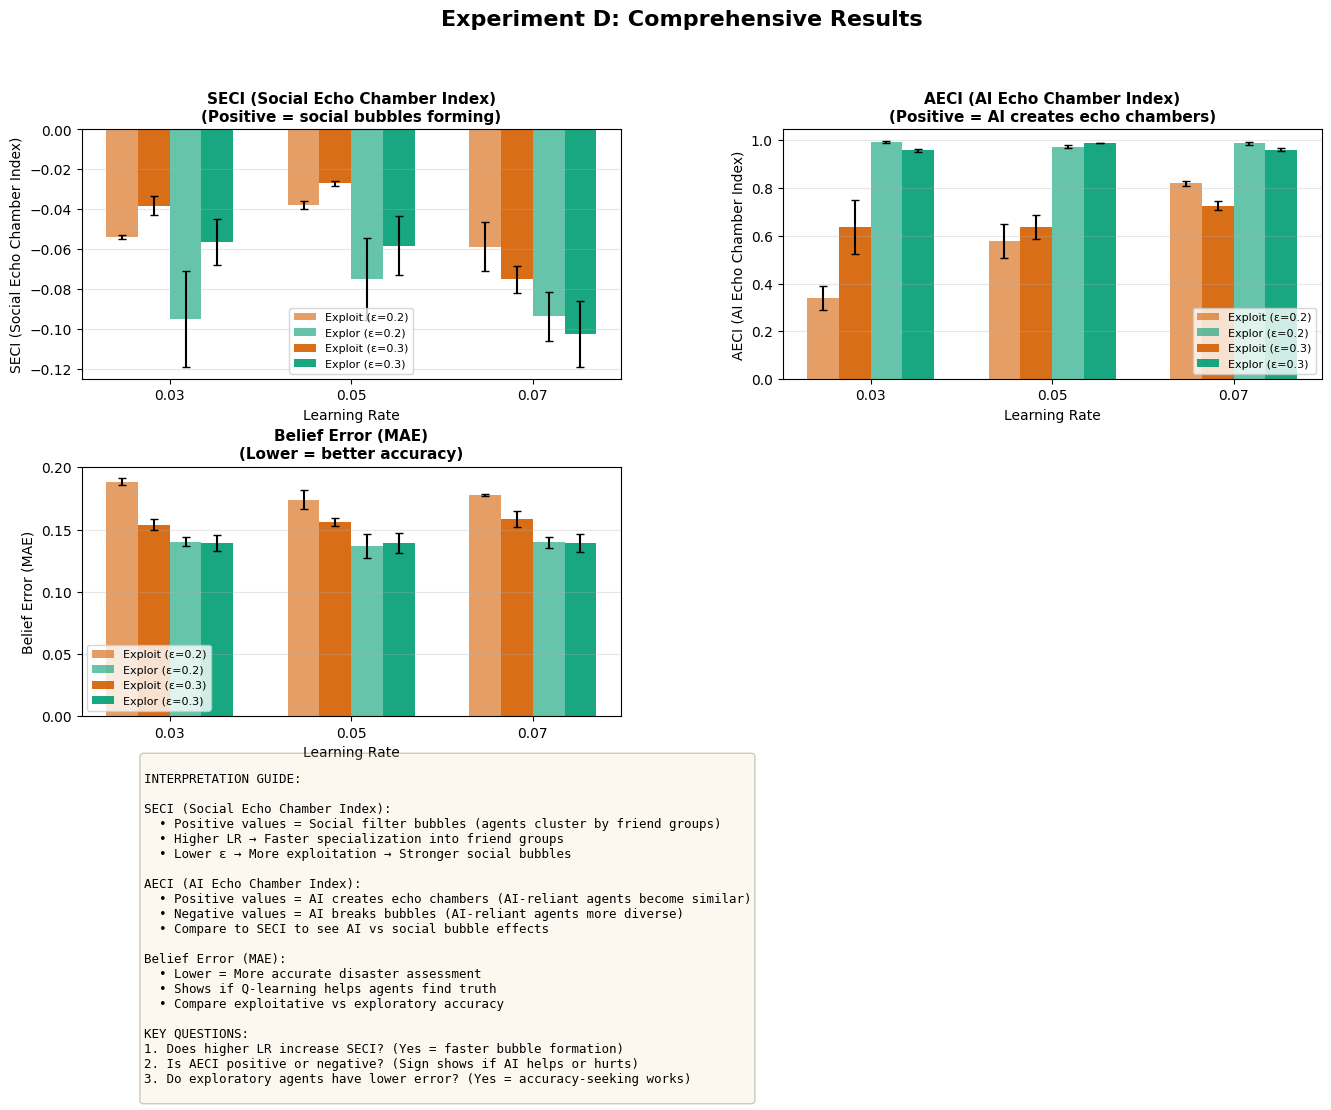
\includegraphics[width=0.5\linewidth]{exp_d_rumor07_AICorrect.png}
    \caption{Enter Caption}
    \label{fig:placeholder}
\end{figure}
\section{Methods}

This paper aims to explore how heterogeneous information sources and dynamic trust relationships influence collective decision-making in disaster response. To this end, an agent-based model is built that combines opinion dynamics frameworks with a decision-making framework that explores the opportunities and challenges of human-AI interaction in crises. The model simulate decentralised disaster relief efforts where human agents, characterized by distinct behavioural types, interact with AI information sources to allocate emergency resources in a spatial environment.

To address these gaps, an agent-based model (ABM) is used to simulate decentralised disaster relief efforts where human agents, characterized by distinct behavioural types, interact with human or AI information sources to allocate emergency resources across a spatial environment. The model expands on established opinion dynamics frameworks \citep{geschke2019triple} to incorporate the challenges of human-AI interaction in crisis contexts.
This computational approach allows us to analyze the trade-offs between the adoption and use of AI and the resulting situational awareness, filter bubbles, and decision performance. By identifying tipping points where AI transitions from mitigating to amplifying filter bubbles, we contribute critical insights to the ongoing discussions about what constitutes trustworthy AI, and how to balance optimization for different objectives in complex and morally charged crisis management scenarios.

\section{Modelling Framework}

The simulation is situated on a 30×30 grid where disaster severity varies from level 0 (no damage) to level 5 (critical need). Human agents of two behavioural types—exploitative and exploratory—navigate this environment alongside AI agents that provide variable-quality information. The model proceeds in discrete time steps where agents sequentially sense their environment, gather information, and allocate relief tokens to perceived high-need locations.

The choice of Q-learning for source selection and Bayesian updates for belief revision represents a novel integration of reinforcement learning and probabilistic reasoning in opinion dynamics modeling. While traditional opinion dynamics models such as \citet{deffuant2000mixing} and \citet{hegselmann2002opinion} typically assume simple averaging or bounded confidence mechanisms, our approach captures the strategic dimension of information seeking and the uncertainty inherent in emergency decision-making. This methodology bridges classic models in social physics with contemporary frameworks for modeling human-AI interaction systems.

\subsection{Agent Architecture}

Human agents maintain cognitive representations comprising individual belief maps about disaster severity across all grid locations and trust profiles for each potential information source. Each agent operates with a Q-learning table that encodes the expected value of consulting different sources, while trust values reflect historical accuracy and reliability assessments. The distinction between exploitative and exploratory agent types emerges from their environmental sensing strategies—exploitative agents prioritize known high-need areas with smaller sensing radii, while exploratory agents employ broader scanning patterns to reduce uncertainty in their belief maps.

AI agents complement this system by periodically sensing random portions of the environment. Their reporting accuracy depends on an alignment parameter that modulates truthfulness, introducing a key experimental variable for examining human-AI trust dynamics. The AI knowledge coverage varies spatially, creating situations where certain regions are better represented in AI information pools than others.

\subsection{Information Diffusion Mechanisms}

The model's information flow follows established principles from opinion dynamics while incorporating strategic behaviour through reinforcement learning. When selecting information sources, agents employ an $\epsilon$-greedy strategy that balances exploration of new sources with exploitation of trusted relationships. Exploitative agents exhibit a structural bias toward consulting friends—implemented through social network analysis—while exploratory agents demonstrate greater willingness to sample diverse sources including AI systems.
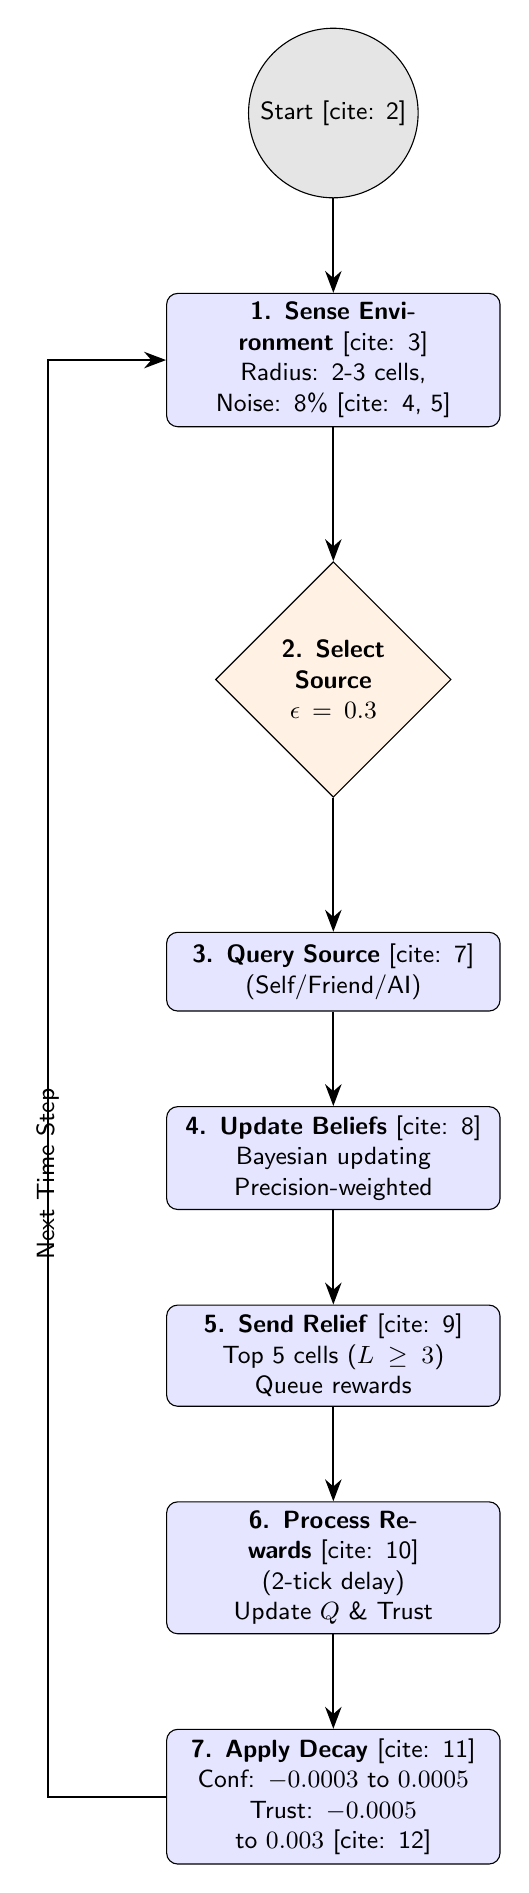
\begin{tikzpicture}[
    node distance=1.2cm and 2cm,
    every node/.style={font=\sffamily\small, align=center},
    process/.style={rectangle, draw, fill=blue!10, text width=4cm, minimum height=1cm, rounded corners},
    decision/.style={diamond, draw, fill=orange!10, text width=2cm, inner sep=0pt},
    data/.style={rectangle, draw=none, fill=none, text width=4cm, font=\sffamily\scriptsize\itshape},
    arrow/.style={-{Stealth[scale=1.2]}, thick}
]

% Nodes based on Figure 2 
\node (start) [circle, draw, fill=gray!20] {Start [cite: 2]};

% 1. Sense Environment
\node (step1) [process, below=of start] {\textbf{1. Sense Environment} [cite: 3] \\ Radius: 2-3 cells, Noise: 8\% [cite: 4, 5]};

% 2. Select Source
\node (step2) [decision, below=of step1, yshift=-0.5cm] {\textbf{2. Select Source}  \\ $\epsilon=0.3$};

% 3. Query Source
\node (step3) [process, below=of step2, yshift=-0.5cm] {\textbf{3. Query Source} [cite: 7] \\ (Self/Friend/AI)};

% 4. Update Beliefs
\node (step4) [process, below=of step3] {\textbf{4. Update Beliefs} [cite: 8] \\ Bayesian updating \\ Precision-weighted};

% 5. Send Relief
\node (step5) [process, below=of step4] {\textbf{5. Send Relief} [cite: 9] \\ Top 5 cells ($L \ge 3$) \\ Queue rewards};

% 6. Process Rewards
\node (step6) [process, below=of step5] {\textbf{6. Process Rewards} [cite: 10] \\ (2-tick delay) \\ Update $Q$ \& Trust};

% 7. Apply Decay
\node (step7) [process, below=of step6] {\textbf{7. Apply Decay} [cite: 11] \\ Conf: $-0.0003$ to $0.0005$ \\ Trust: $-0.0005$ to $0.003$ [cite: 12]};

% Arrows
\draw [arrow] (start) -- (step1);
\draw [arrow] (step1) -- (step2);
\draw [arrow] (step2) -- (step3);
\draw [arrow] (step3) -- (step4);
\draw [arrow] (step4) -- (step5);
\draw [arrow] (step5) -- (step6);
\draw [arrow] (step6) -- (step7);

% Feedback Loop for the "Cycle"
\draw [arrow] (step7.west) -- ++(-1.5,0) |- (step1.west) 
    node[pos=0.25, left, rotate=90] {Next Time Step};

\end{tikzpicture}

Belief updating employs Bayesian inference with agent-type-specific priors, extending classical consensus models through heterogeneous resistance to belief change. The update mechanism weighs new information according to source trust and existing confidence levels, with precision-based formulations that naturally handle conflicting reports. This approach aligns with recent developments in modeling opinion dynamics under uncertainty \citep{lorenz2017continuous} while incorporating the computational constraints of emergency response scenarios.

\subsection{Trust Evolution}

Trust dynamics emerge from two parallel processes: direct observation of information accuracy and reinforcement learning based on assistance outcomes. The trust update mechanism combines immediate feedback from ground truth comparisons with delayed rewards from relief allocation effectiveness. This dual-track approach captures both the cognitive updating of source reliability assessments and the pragmatic evaluation of information utility for decision support.

The model introduces asymmetric trust learning rates for different agent types and source categories. Exploitative agents exhibit higher initial trust in AI systems when alignment is high, while exploratory agents demonstrate inverse sensitivity—trusting AI more when alignment suggests truthful reporting. This behavioral heterogeneity produces emergent trust polarization that significantly influences collective performance metrics.

\subsection{Echo Chamber Quantification}

The Social Echo Chamber Index (SECI) measures within-group belief homogeneity relative to population-wide variance, following established approaches in network opinion dynamics. The AI Echo Chamber Index (AECI) introduces a novel metric combining usage frequency with belief variance reduction among AI-reliant agents. Component-level analysis extends these metrics to identify localized consensus clusters arising from network topology.

SECI quantifies belief similarity within social groups through variance comparison:

\begin{equation}
SECI = \frac{V_{global} - V_{friend}}{V_{global}}
\end{equation}

where belief variance within friend groups ($V_{friend}$) is compared against global population variance. Higher values indicate stronger echo chambers.

AECI captures both behavioral patterns and belief convergence:

\begin{equation}
AECI_{behavioral} = P(query_{AI})
\end{equation}

\begin{equation}
AECI_{variance} = \frac{V_{global} - V_{AI-reliant}}{V_{global}}
\end{equation}

These indices reveal how information source preferences translate into measurable belief clustering, with network topology playing a crucial moderating role.

\subsection{Relief Allocation and Performance Evaluation}

Agents allocate relief tokens to cells based on weighted combinations of perceived severity and belief confidence. Exploitative agents prioritize confidence-weighted severity, while exploratory agents balance severity assessment with uncertainty reduction objectives. Token placement effectiveness is evaluated through delayed reward signals that compare allocated resources against actual need distributions.

The performance metrics encompass assistance accuracy (correctly targeted high-need cells), belief error (mean absolute deviation from ground truth), and coverage of critical needs. These measures capture both the efficiency and equity dimensions of disaster response, crucial for evaluating information flow impacts on collective outcomes.

\subsection{Experimental Framework}

The study implements three core experiments examining agent composition effects, AI alignment sensitivity, and environmental dynamics. Agent mix variations test how the ratio of exploitative to exploratory types influences system performance. AI alignment experiments probe for tipping points where agent preferences shift between human and AI information sources. Environmental dynamics investigations vary disaster intensity and shock frequency to assess system robustness.

Each experiment runs 20 replications to capture stochastic variation, with Monte Carlo sampling of initial conditions including agent placement, social network structure, and belief initialization. Statistical analysis employs non-parametric methods to handle non-normal performance distributions, while time series analysis tracks evolution of trust and belief metrics throughout crisis scenarios.

\subsection{Technical Implementation}

Model implementation utilizes the Mesa framework for agent-based modeling, with belief updating optimized for computational efficiency through vectorized operations. Network analysis employs NetworkX for component detection and social structure analysis. Visualization tools include real-time belief maps, trust evolution trackers, and performance dashboards for experimental monitoring.

Parameter sensitivity analysis revealed robust performance across a range of learning rates (0.01-0.1) and confidence thresholds, with critical dependencies on trust learning rates and network topology. These findings inform practical applications while highlighting theoretical relationships between information structure and collective decision quality in crisis scenarios.

\section{Results}\label{sec2}

Sample body text. Sample body text. Sample body text. Sample body text. Sample body text. Sample body text. Sample body text. Sample body text.

\section{This is an example for first level head---section head}\label{sec3}

\subsection{This is an example for second level head---subsection head}\label{subsec2}

\subsubsection{This is an example for third level head---subsubsection head}\label{subsubsec2}

Sample body text. Sample body text. Sample body text. Sample body text. Sample body text. Sample body text. Sample body text. Sample body text. 



\section{Discussion}\label{sec12}

Discussions should be brief and focused. In some disciplines use of Discussion or `Conclusion' is interchangeable. It is not mandatory to use both. Some journals prefer a section `Results and Discussion' followed by a section `Conclusion'. Please refer to Journal-level guidance for any specific requirements. 

\section{Conclusion}\label{sec13}

Conclusions may be used to restate your hypothesis or research question, restate your major findings, explain the relevance and the added value of your work, highlight any limitations of your study, describe future directions for research and recommendations. 

In some disciplines use of Discussion or 'Conclusion' is interchangeable. It is not mandatory to use both. Please refer to Journal-level guidance for any specific requirements. 

\backmatter

\bmhead{Supplementary information}

If your article has accompanying supplementary file/s please state so here. 

Authors reporting data from electrophoretic gels and blots should supply the full unprocessed scans for key as part of their Supplementary information. This may be requested by the editorial team/s if it is missing.

Please refer to Journal-level guidance for any specific requirements.

\bmhead{Acknowledgements}

Acknowledgements are not compulsory. Where included they should be brief. Grant or contribution numbers may be acknowledged.

Please refer to Journal-level guidance for any specific requirements.

\section*{Declarations}

Some journals require declarations to be submitted in a standardised format. Please check the Instructions for Authors of the journal to which you are submitting to see if you need to complete this section. If yes, your manuscript must contain the following sections under the heading `Declarations':

\begin{itemize}
\item Funding
\item Conflict of interest/Competing interests (check journal-specific guidelines for which heading to use)
\item Ethics approval and consent to participate
\item Consent for publication
\item Data availability 
\item Materials availability
\item Code availability 
\item Author contribution
\end{itemize}

\noindent
If any of the sections are not relevant to your manuscript, please include the heading and write `Not applicable' for that section. 

%%===================================================%%
%% For presentation purpose, we have included        %%
%% \bigskip command. Please ignore this.             %%
%%===================================================%%
\bigskip
\begin{flushleft}%
Editorial Policies for:

\bigskip\noindent
Springer journals and proceedings: \url{https://www.springer.com/gp/editorial-policies}

\bigskip\noindent
Nature Portfolio journals: \url{https://www.nature.com/nature-research/editorial-policies}

\bigskip\noindent
\textit{Scientific Reports}: \url{https://www.nature.com/srep/journal-policies/editorial-policies}

\bigskip\noindent
BMC journals: \url{https://www.biomedcentral.com/getpublished/editorial-policies}
\end{flushleft}

\begin{appendices}
\section{Bayesian Belief Update Formalisation}

The belief update mechanism chosen in this paper extends the traditional Bayesian inference \citep{schneider2025emergency} by explicitly distinguishing two agent types and adjusting the respective resistance parameters and trust-weighted information integration. When agent $i$ receives information about cell $(x,y)$ from source $j$, the update follows:

\begin{equation}
precision_{prior}^{i,j} = \frac{\alpha_i \cdot conf_i}{ 1 - conf_i + \epsilon}
\end{equation}

\begin{equation}
precision_{source}^{i,j} = \frac{\beta_{i,j} \cdot trust_{i,j}}{1 - trust_{i,j} + \epsilon}
\end{equation}

where $\alpha_i \in \{0.8, 1.8\}$ for exploratory and exploitative agents respectively, and $\beta_{i,j} \in \{2.5, 4.0\}$ distinguishes between agent types. The posterior belief emerges as:

\begin{equation}
L_{posterior} = \frac{L_{prior} \cdot precision_{prior} + L_{reported} \cdot precision_{source}}{precision_{prior} + precision_{source}}
\end{equation}

\begin{equation}
conf_{posterior} = \frac{precision_{prior} + precision_{source}}{1 + precision_{prior} + precision_{source}}
\end{equation}

Confirmation effects are modeled through type-specific boosts: when $|L_{posterior} - L_{prior}| \leq 1$:
\begin{itemize}
   \item Exploitative agents: $conf_{posterior} \leftarrow \min(0.98, conf_{posterior} + 0.35 \cdot conf_{prior})$
   \item Exploratory agents: minimal adjustment to preserve information openness
\end{itemize}

This formulation draws from work on bounded-confidence models \citep{deffuant2000mixing} and incorporates motivated reasoning patterns documented in social psychology \citep{kunda1990case}.

\section{Q-Learning Architecture}

The Q-learning implementation balances classical temporal difference methods with domain-specific modifications for emergency response:

State representation $s = \{interest\_point, source\_history, trust\_vector\}$

Action space $A = \{self, friend, A_0, ..., A_4\}$ with exploitative agents receiving biased action values:
\begin{itemize}
   \item Friend bias: $Q_{exploit}(a_{friend}) \leftarrow Q(a_{friend}) + 0.1$
   \item Self-confirmation bias: $Q_{exploit}(a_{self}) \leftarrow Q(a_{self}) + 0.1$
\end{itemize}

Reward structure incorporates both immediate accuracy and delayed assistance effectiveness:

\begin{equation}
R_t = \begin{cases}
5.0 & \text{if } L_{true} = 5 \text{ (critical need)} \\
3.0 & \text{if } L_{true} = 4 \\
1.5 & \text{if } L_{true} = 3 \\
-1.0 & \text{if } L_{true} = 1 \\
-2.0 & \text{if } L_{true} = 0
\end{cases}
\end{equation}

Agent-type-specific Q-value updates:
\begin{itemize}
   \item Exploratory: $Q(s,a) \leftarrow Q(s,a) + \alpha (0.8 \cdot R_{actual} + 0.2 \cdot R_{correctness} - Q(s,a))$
   \item Exploitative: $Q(s,a) \leftarrow Q(s,a) + \alpha (0.2 \cdot R_{actual} + 0.8 \cdot R_{correctness} - Q(s,a))$
\end{itemize}

This design connects to reinforcement learning literature in social systems \citep{shoham2003multi} while addressing the specific challenges of multi-source information environments.

\section{Trust Evolution Dynamics}

Trust update mechanism combines immediate accuracy feedback with long-term utility assessment:

\begin{equation}
\Delta trust_{i,j}^{immediate} = learning\_rate_{accuracy} \cdot (1 - |L_{actual} - L_{believed}|/5)
\end{equation}

\begin{equation}
\Delta trust_{i,j}^{delayed} = learning\_rate_{utility} \cdot \frac{R + 1}{2}
\end{equation}

Agent-type learning rates introduce asymmetric adaptation:
\begin{itemize}
   \item Exploitative towards AI: $lr_{AI} = 0.03 \rightarrow 0.03 \cdot (1 + alignment)$
   \item Exploratory towards AI: $lr_{AI} = 0.08 \rightarrow 0.08 \cdot (1 + (1-alignment) \cdot 1.5)$
\end{itemize}

Trust decay incorporates relationship proximity:
\begin{itemize}
   \item Friend decay: $decay = 0.0005$ (exploitative), $0.0015$ (exploratory)
   \item Non-friend decay: $decay = 0.002$ (base)
   \item AI decay: $decay \cdot (1 - alignment \cdot 0.5)$ for appropriately skeptical agents
\end{itemize}

This approach is in line with modelling trust in human-AI teams \citep{lee2004trust,gambetta2005streetwise}.

\section{Rumor Propagation Architecture}

Rumour initialisation employs component-wise seeding with spatial constraints:

For each network component $C_i$ with probability $p_{rumor} = 0.7$:

\begin{equation}
epicenter_{rumor} \sim Uniform(grid) \quad s.t. \quad ||epicenter_{rumor} - epicenter_{true}|| > r_{disaster} \cdot 0.5
\end{equation}

Rumour intensity follows Gaussian decay:
\begin{equation}
L_{rumor}(x,y) = \min(5, 3 + intensity) \cdot e^{-\frac{d(x,y)^2}{2\sigma_{rumor}^2}}
\end{equation}

where $\sigma_{rumor} = r_{disaster} \cdot 0.5$ and $d(x,y)$ denotes distance from rumor epicenter. Initial confidence varies:
\begin{equation}
conf_{rumor} = conf_{base} + \mathcal{N}(0, 0.1)
\end{equation}

This formalization extends epidemiological models of misinformation spread \citep{vosoughi2018spread} to spatial disaster contexts.

\section{Echo Chamber Measurement Framework}

Component SECI analysis partitions agents by network connectivity:
\begin{equation}
SECI_{component\_k} = \frac{V_{global} - V_{component\_k}}{V_{global}}
\end{equation}

AECI-variance tracks belief convergence among AI-reliant agents:
\begin{equation}
AECI_{variance} = max(0, \frac{V_{global} - V_{AI-reliant}}{V_{global}})
\end{equation}

where $AI-reliant = \{agents: ratio_{AI\_calls} > 0.2\}$ with $\geq 3$ total calls.

Component AI trust variance measures trust clustering within components:
\begin{equation}
V_{trust,k} = Var(\{\overline{trust}_{AI}^{i} : i \in C_k\})
\end{equation}

These metrics extend established approaches in network opinion dynamics \citep{friedkin1999social} while capturing specific phenomena in human-AI information systems.

\bibliography{References}



\end{appendices}

%%===========================================================================================%%
%% If you are submitting to one of the Nature Portfolio journals, using the eJP submission   %%
%% system, please include the references within the manuscript file itself. You may do this  %%
%% by copying the reference list from your .bbl file, paste it into the main manuscript .tex %%
%% file, and delete the associated \verb+\bibliography+ commands.                            %%
%%===========================================================================================%%

\bibliography{sn-bibliography}% common bib file
%% if required, the content of .bbl file can be included here once bbl is generated
%%\input sn-article.bbl

\end{document}
